% Harus dimuat terlebih dahulu, digunakan agar file PDF memiliki format karakter yang benar.
% Untuk informasi lebih lanjut, lihat https://ctan.org/pkg/cmap.
\RequirePackage{cmap}

% Format dokumen sebagai paper konferensi menggunakan aturan IEEEtran terbaru (v1.8b).
% Untuk informasi lebih lanjut, lihat http://www.michaelshell.org/tex/ieeetran/.
\documentclass[conference]{IEEEtran}

% Format encoding font dan input menjadi 8-bit UTF-8.
\usepackage[T1]{fontenc}
\usepackage[utf8]{inputenc}
\usepackage{amsmath}
% Digunakan untuk mengatur margin dokumen.
\usepackage{textcomp}

% Digunakan untuk tujuan demonstrasi.
\usepackage{mwe}

% Digunakan untuk menampilkan font dengan style yang lebih baik.
\usepackage[zerostyle=b,scaled=.75]{newtxtt}

% Digunakan untuk menampilkan tabel dengan style yang lebih baik.
\usepackage{booktabs}
\usepackage[table,xcdraw]{xcolor}

% Digunakan untuk menampilkan gambar pada dokumen.
\usepackage{graphicx}
\usepackage{float}

% Digunakan untuk menampilkan potongan kode.
\usepackage{listings}
\lstset{
  basicstyle=\ttfamily,
  columns=fixed,
  basewidth=.5em,
  xleftmargin=0.5cm,
  captionpos=b
}

\usepackage{tabularx}
\usepackage{wrapfig}
% Digunakan agar backticks (`) dapat dirender pada PDF.
% Untuk informasi lebih lanjut, lihat https://tex.stackexchange.com/a/341057/9075.
\usepackage{upquote}

% Digunakan untuk menyeimbangkan bagian akhir dokumen dengan dua kolom.
\usepackage{balance}

% Digunakan untuk menampilkan pustaka.
\usepackage[square,comma,numbers,sort&compress]{natbib}

% Mengubah format ukuran teks pada natbib.
\renewcommand{\bibfont}{\normalfont\footnotesize}

% Jika melebihi 3 penulis dapat dilakukan linebreakend 
\makeatletter
\newcommand{\linebreakand}{%
  \end{@IEEEauthorhalign}
  \hfill\mbox{}\par
  \mbox{}\hfill\begin{@IEEEauthorhalign}
}
\makeatother

% Menambah nama penulis ketika menggunakan perintah \citet.
% Untuk informasi lebih lanjut, lihat https://tex.stackexchange.com/a/76075/9075.
\usepackage{etoolbox}
\makeatletter
\patchcmd{\NAT@test}{\else \NAT@nm}{\else \NAT@hyper@{\NAT@nm}}{}{}
\makeatother

% Digunakan untuk melakukan linewrap pada pustaka dengan url yang panjang
% jika terdapat hyphens
\usepackage[hyphens]{url}

% Digunakan untuk menambah hyperlink pada referensi.
\usepackage{hyperref}

% Menonaktifkan warna dan bookmark pada hyperref.
\hypersetup{hidelinks,
  colorlinks=true,
  allcolors=black,
  pdfstartview=Fit,
  breaklinks=true
}

% Digunakan untuk membenarkan hyperref pada gambar.
\usepackage[all]{hypcap}

% Digunakan untuk menampilkan beberapa gambar
\usepackage[caption=false,font=footnotesize]{subfig}

\usepackage{stfloats}
% nama
\newcommand{\name}{Moh. Iqbal Fatchurozi}
\newcommand{\authorname}{Fatchurozi, Moh. Iqbal}
\newcommand{\nickname}{Iqbal}
\newcommand{\advisor}{Arief Kurniawan}
\newcommand{\coadvisor}{Eko Mulyanto Yuniarno}

% identitas
\newcommand{\nrp}{5024 20 1009}
\newcommand{\advisornip}{19740907 200212 1 001}
\newcommand{\coadvisornip}{19680601 199512 1 009}
\newcommand{\email}{5024201009@student.its.ac.id}
\newcommand{\advisoremail}{arifku@ee.its.ac.id}
\newcommand{\coadvisoremail}{ekomulyanto@ee.its.ac.id}

% judul
\newcommand{\tatitle}{Judul Paper}
\newcommand{\engtatitle}{Paper Title}

% tempat
\newcommand{\place}{Surabaya}

% jurusan
\newcommand{\studyprogram}{Teknik Komputer}
\newcommand{\engstudyprogram}{Computer Engineering}

% fakultas
\newcommand{\faculty}{Teknologi Elektro dan Informatika Cerdas}
\newcommand{\engfaculty}{Intelligence Electrical and Informatics Technology}

% singkatan fakultas
\newcommand{\facultyshort}{FTEIC}
\newcommand{\engfacultyshort}{ELECTICS}

% departemen
\newcommand{\department}{Teknik Komputer}
\newcommand{\engdepartment}{Computer Engineering}

% Tambahkan format tanda hubung yang benar di sini
\hyphenation{
  ro-ket
  me-ngem-bang-kan
  per-hi-tu-ngan
}


\begin{document}

% Ubah kalimat berikut sesuai dengan judul penelitian.
\title{\engtatitle{}}

% Ubah kalimat-kalimat berikut sesuai dengan nama, institusi, alamat dan kontak penulis.
\author{
  \IEEEauthorblockN{\name{}}
  \IEEEauthorblockA{\textit{dept. of \engstudyprogram{}}\\
    \textit{Institut Teknologi Sepuluh Nopember}\\
    Surabaya, Indonesia 60111\\
    \email{}}

  \and
  \IEEEauthorblockN{\advisor{}}
  \IEEEauthorblockA{\textit{dept. of \engstudyprogram{}}\\
    \textit{Institut Teknologi Sepuluh Nopember}\\
    Surabaya, Indonesia 60111\\
    \advisoremail{}}

  \and
  \IEEEauthorblockN{\coadvisor{}}
  \IEEEauthorblockA{\textit{dept. of \engstudyprogram{}}\\
    \textit{Institut Teknologi Sepuluh Nopember}\\
    Surabaya, Indonesia 60111\\
    \coadvisoremail{}}
}

% Digunakan untuk menampilkan judul dan deskripsi penulis.
\maketitle

% Mengubah keterangan `Abstract` ke bahasa indonesia.
% Hapus bagian ini untuk mengembalikan ke format awal.
% \renewcommand\abstractname{Abstrak}

\begin{abstract}

  % Ubah paragraf berikut sesuai dengan abstrak dari penelitian.
  This thesis presents a novel approach to enhancing mobility for ALS patients by developing
  a wheelchair movement control system using MediaPipe, centered on eye gesture recognition,
  and implemented on a Jetson Nano platform. The study is motivated by the challenges faced
  by ALS patients who, despite losing physical mobility, retain the ability to move their eyes. The
  proposed system aims to provide these individuals with increased independence and improved
  quality of life. The methodology comprises several key components: capturing and processing
  eye images, extracting relevant features, estimating and classifying eye positions, and executing
  the control system on a Next Unit of Computing (NUC). The integration of computer vision
  technology with an embedded system is a cornerstone of this research, ensuring a responsive
  and efficient wheelchair control mechanism. By leveraging the power of MediaPipe for
  real-time gesture recognition and the computational capabilities of Jetson Nano, the study
  promises to significantly enhance the autonomy of wheelchair users with mobility impairments.
  This research not only contributes to the field of assistive technology but also serves as a
  potential model for future innovations in mobility solutions for individuals with various physical
  disabilities.


\end{abstract}

% Mengubah keterangan `Index terms` ke bahasa indonesia.
% Hapus bagian ini untuk mengembalikan ke format awal.
% \renewcommand\IEEEkeywordsname{Kata kunci}

\begin{IEEEkeywords}

  % Ubah kata-kata berikut sesuai dengan kata kunci dari penelitian.
  Assistive Technology, Gesture Recognition, Wheelchair Control

\end{IEEEkeywords}


% Ubah bagian berikut sesuai dengan konten-konten yang akan dimasukkan pada dokumen
% Ubah judul dan label berikut sesuai dengan yang diinginkan.
\section{Introduction}
\label{sec:introduction}

% Ubah paragraf-paragraf pada bagian ini sesuai dengan yang diinginkan.
Disabilitas adalah kondisi dimana tubuh atau pikiran terganggu yang membuat orang dengan kondisi tersebut lebih sulit melakukan aktivitas tertentu dan lebih sulit untuk berinteraksi dengan dunia di sekelilingnya \cite{CDC_2020}. Menurut \textit{World Health Organization}, disabilitas adalah bagian dari diri manusia dan merupakan bagian yang tidak terpisahkan dari pengalaman manusia. Hal ini merupakan hasil dari interaksi antara kondisi kesehatan seperti demensia, kebutaan atau cedera tulang belakang, dan berbagai faktor lingkungan dan pribadi. Diperkirakan 1,3 miliar orang - atau 16\% dari populasi global - mengalami disabilitas yang signifikan saat ini. Jumlah ini terus bertambah karena meningkatnya penyakit tidak menular dan orang yang hidup lebih lama \cite{WHO_2023}.

Salah satu kondisi yang dapat menyebabkan disabilitas yaitu tetraplegia merupakan salah satu kondisi cedera tulang belakang dimana manusia hanya dapat menggerakkan bagian tubuh bagian atas, seperti kepala, leher, dan bahu. Salah satu penyakit yang termasuk dalam kondisi tetraplegia adalah \textit{Amyotrophic Lateral Sclerosis} atau yang biasa disingkat ALS. \textit{Amyotrophic lateral sclerosis} atau ALS, yang sebelumnya dikenal sebagai penyakit Lou Gehrig, adalah kelainan neurologis yang memengaruhi neuron motorik, yaitu sel-sel saraf di otak dan sumsum tulang belakang yang mengontrol gerakan otot dan pernapasan. Ketika neuron motorik mengalami degenerasi dan mati, neuron motorik berhenti mengirimkan pesan ke otot, yang menyebabkan otot melemah, mulai berkedut (fasikulasi), dan mengecil (atrofi). Pada akhirnya, pada penderita ALS, otak kehilangan kemampuannya untuk memulai dan mengontrol gerakan otot yang dibutuhkan untuk berjalan, berbicara, mengunyah dan fungsi lainnya, serta bernapas. ALS bersifat progresif, yang berarti gejalanya memburuk dari waktu ke waktu \cite{NINDS}. 

Dalam stadium terakhir penyakit ALS, dimana rata-rata waktu dalam dua hingga lima tahun \cite{ALS_2023}, pasien ALS biasanya kehilangan kemampuan gerakan fisik termasuk berbicara dan menulis tangan, tetapi untungnya mereka masih bisa menggerakkan mata mereka \cite{Eyesay_2023}. Oleh sebab itu, pasien ALS perlu pendamping dalam melakukan aktivitas sehari-hari, namun ada saatnya dimana mereka harus bisa beraktivitas secara mandiri. Dalam hal tersebut, mereka membutuhkan kursi roda untuk bergerak dalam melakukan aktivitas sehari-hari. Di sisi lain, kursi roda elektrik yang ada pada saat ini, bergantung pada lengan atas pengguna untuk kontrol yang menyulitkan pasien tetraplegia untuk mengendalikannya \cite{9935646}. 

Untuk mengatasi permasalahan tersebut, penting untuk mencari solusi untuk dapat mempermudah sistem kontrol kursi roda sehingga dapat meningkatkan kemandirian pasien ALS. Pendekatan yang menjanjikan adalah pemanfaatan teknologi visi komputer dan sistem tertanam. Visi komputer memungkinkan komputer untuk "melihat" dan memproses citra \cite{TIAN20201}, teknologi ini menggunakan kamera untuk mengidentifikasi, melacak, hingga mengukur target untuk pemrosesan citra lebih lanjut. Visi komputer memberikan kemampuan untuk mengenali dan memahami lingkungan sekitar. Penting untuk menggunakan perangkat keras yang sesuai untuk tujuan tersebut. Baru-baru ini, model pengenalan gambar telah ditanam pada platform target yang sebenarnya, yang merupakan komputer dengan tujuan khusus, seperti perangkat IoT seluler atau kendaraan otonom, dan bukan pada server atau PC yang digunakan di laboratorium. Sistem tertanam umumnya digunakan di lapangan, namun ada persyaratan operasional untuk lingkungan, ukuran fisik, dll \cite{8939843}. Dengan menggabungkan kedua teknologi tersebut, maka pada penelitian ini memberikan solusi yaitu dengan mengembangkan sistem kontrol pergerakan kursi roda yang dapat dikendalikan melalui gerakan mata.

Dalam mewujudkan solusi tersebut, maka penelitian ini difokuskan untuk mengembangkan sistem kontrol kursi roda yang dapat berinteraksi dengan teknologi visi komputer dalam sistem tertanam. NUC \textit{(Next Unit of Computing)} adalah pilihan yang tepat untuk pengembangan sistem tertanam karena efektivitas biaya, kemudahan penggunaan, dan fleksibilitas. Penelitian ini diharapkan dapat menciptakan sistem kontrol kursi roda yang efisien dan responsif dalam mengatasi masalah mobilitas pada penderita ALS.
% Ubah judul dan label berikut sesuai dengan yang diinginkan.
\section{Literature Review}
\label{sec:relatedworks}

\subsection{Electric Wheelchair}
A wheelchair is a manually operated or power-driven device designed primarily for use by individuals with mobility disabilities for the primary purpose of moving indoors, or indoors and outdoors.  Individuals with mobility disabilities must be permitted to use wheelchairs and manually powered mobility aids, such as walkers, crutches, canes, or other similar devices designed for use by individuals with mobility disabilities, in any area open to pedestrian traffic \cite{ADA_2023}. An electric wheelchair can be seen in Figure \ref{fig:kursiroda}.

%Gambar 2.1
% Contoh input gambar
\begin{figure}[ht]
  \centering

  % Ubah dengan nama file gambar dan ukuran yang akan digunakan
  \includegraphics[scale=0.2]{gambar/bab3/wheel.jpeg}

  % Ubah dengan keterangan gambar yang diinginkan
  \caption{Electric Wheelchair}
  \label{fig:kursiroda}
\end{figure}

\subsection{Eye Gesture}

Eye gesture refers to eye movements, such as eye gaze, eye pose, and facial expressions, which play an important role in human communication and interaction. Eye tracking devices have been used to study various aspects of eye pose, including the influence of social factors, physical factors, and the relationship between eye pose and speech. These devices can record participants' eye poses with a corneal reflex camera and analyze body pose and eye pose with temporal accuracy \cite{gullberg_kita_2009}. An example of an eye pose can be seen in Figure \ref{fig:gaze}.

% Gambar 2.2
\begin{figure} [ht] \centering
    % Nama dari file gambar yang diinputkan
    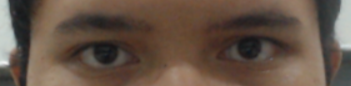
\includegraphics[scale=0.5]{gambar/bab3/gaze.png}
    % Keterangan gambar yang diinputkan
    \caption{Eye Pose}
    % Label referensi dari gambar yang diinputkan
    \label{fig:gaze}
\end{figure}

\subsection{MediaPipe Face Mesh}

MediaPipe Face Mesh is a face landmark detection solution that estimates 468 3D face landmarks in real-time, even on mobile devices. The solution utilizes a pipeline of two neural networks to identify 3D coordinates of facial landmarks from 2D images. The first network, BlazeFace, calculates the location of the face from the full image, while the second network operates on the cropped region to identify the location of the landmarks \cite{mediapipe_2020}. The technology has a wide range of applications, including face mask detection, hands-free computer control, and gestures accompanying speech \cite{thaman_2022}. A visualization of the MediaPipe Face Mesh can be seen in Figure \ref{fig:facemesh}.

% Gambar 2.3
\begin{figure} [ht] \centering
    % Nama dari file gambar yang diinputkan
    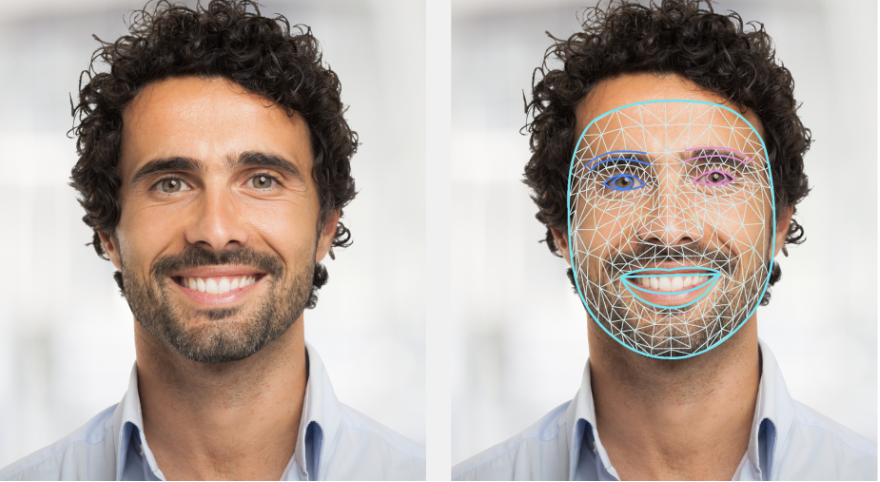
\includegraphics[scale=0.4]{gambar/face_landmark.png}
    % Keterangan gambar yang diinputkan
    \caption{MediaPipe Face Mesh}
    % Label referensi dari gambar yang diinputkan
    \label{fig:facemesh}
\end{figure}

\subsection{Convolutional Neural Network (CNN)}

A Convolutional Neural Network (CNN) is a type of artificial neural network used primarily for image recognition and processing. It is a subset of machine learning and is specifically designed to identify and recognize objects in images, as well as for tasks such as object classification and pattern recognition \cite{arm_2023}. 

The architecture of a CNN consists of three parts, namely input, feature learning, and classification. The Feature Learning consists of two convolution layers and two pooling layers. In classification consists of two hidden layers and one output layer. CNN architecture can be depicted as in Figure \ref{fig:arsitektur cnn}.

% Gambar 2.4
\begin{figure} [ht] \centering
    % Nama dari file gambar yang diinputkan
    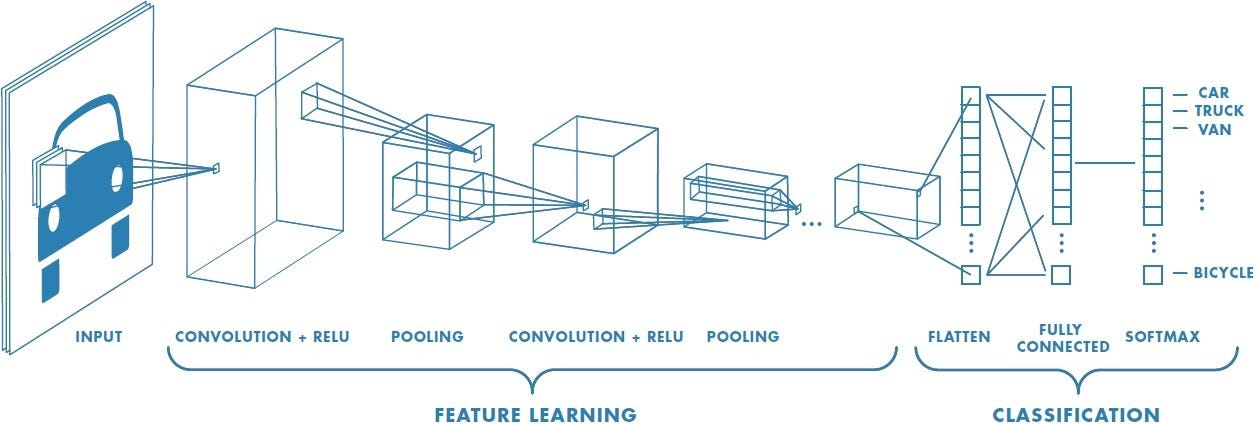
\includegraphics[scale=0.2]{gambar/cnn.jpg}
    % Keterangan gambar yang diinputkan
    \caption{Convolutional Neural Network Architecture}
    % Label referensi dari gambar yang diinputkan
    \label{fig:arsitektur cnn}
\end{figure}

\subsection{Confusion Matrix}

The Confusion Matrix is a tool used to evaluate the performance of classification models in machine learning. It provides a detailed overview of how the classification model works, showing the relationship between the model's predictions and the actual values. The Confusion Matrix is a tabular representation consisting of four main components, namely True Positive (TP), False Positive (FP), True Negative (TN), and False Negative (FN). Each component has a specific meaning in the context of prediction \cite{provost2013data}. The visualization of confusion matrix can be seen in Figure \ref{fig:confusion}.

% Gambar 2.7
\begin{figure} [ht] \centering
    % Nama dari file gambar yang diinputkan
    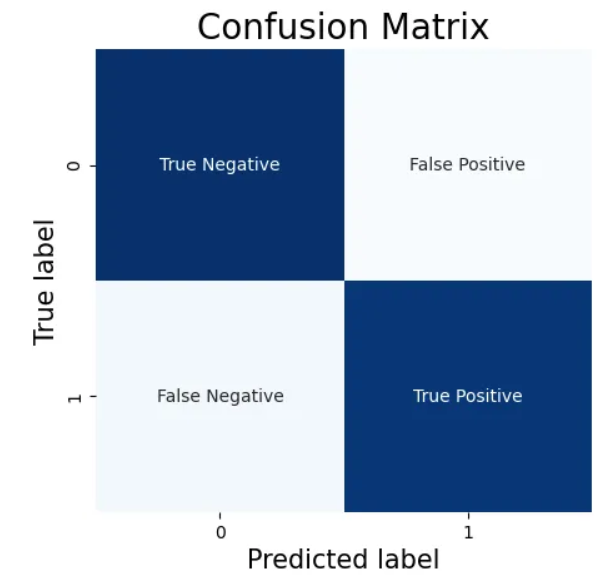
\includegraphics[scale=0.3]{gambar/bab2/confusion.png}
    % Keterangan gambar yang diinputkan
    \caption{Confusion Matrix Visualization}
    % Label referensi dari gambar yang diinputkan
    \label{fig:confusion}
\end{figure}

\subsection{Accuracy}
\label{subsec:acc_klasifikasi}

Accuracy is a performance measure that indicates how correctly the model can classify the test data. In this context, accuracy is the ratio of correct predictions (TP and TN) to the total amount of data. In other words, accuracy measures how close the predicted value is to the actual value. The value of accuracy can be obtained using Equation \ref{eq:acc}.

\begin{equation}
  \label{eq:acc}
  Accuracy=\frac{TP+TN}{TP+TN+FP+FN}
\end{equation}

\subsection{Precision}
\label{subsec:prec_klasifikasi}

Precision is a performance measure that indicates the degree of accuracy of the requested data compared to the predicted results provided by the model. In this context, precision is the ratio of correct positive predictions (TP) to the total positive prediction results (TP and FP). The value of precision can be obtained by Equation \ref{eq:prec}.

\begin{equation}
  \label{eq:prec}
  Precision=\frac{TP}{TP+FP}
\end{equation}

\subsection{Recall}
\label{subsec:recall_klasifikasi}

Recall is a performance measure that indicates how successful the model is in retrieving information. In this context, recall is the ratio between correct positive predictions (TP) and the total number of positive actual data (TP and FN). Thus, the recall value can be calculated using Equation \ref{eq:recall}.

\begin{equation}
  \label{eq:recall}
  Recall=\frac{TP}{TP+FN}
\end{equation}

\subsection{F1-Score}
\label{subsec:score_klasifikasi}

The F1-Score is a value between zero (0) to one (1) obtained from the harmonic mean between the precision value and the recall value. Therefore, the value of F1-Score can be calculated using Equation \ref{eq:score}.

\begin{equation}
  \label{eq:score}
  F{1}{-}Score=\frac{2 \times Precision \times Recall}{Precision+Recall}
\end{equation}

\subsection{Next Unit of Computing (NUC)}

Intel NUC, or Next Unit of Computing, is a mini computer device that has high computing power in a compact form. With its small dimensions, NUC is still able to provide powerful performance for various computing needs. The latest NUC models are equipped with the latest generation of Intel Core processors, support 4K graphics, and have extensive connectivity capabilities such as Thunderbolt, USB, HDMI, and Ethernet. These advantages make it an ideal choice for edge computing applications and applications that require high computing power in a limited space \cite{intel_nuc}.
% Ubah judul dan label berikut sesuai dengan yang diinginkan.
\section{Architecture}
\label{sec:architecture}

% Ubah paragraf-paragraf pada bagian ini sesuai dengan yang diinginkan.

\subsection{Cetak Biru Roket}
\label{subsec:cetakbiruroket}

Pada cetak biru yang tertera pada Gambar \ref{fig:cetakbiru}. \lipsum[8]

% Contoh input gambar pada kolom.
\begin{figure} [ht]
  \centering
  % Ubah sesuai dengan nama file gambar dan ukuran yang akan digunakan.
  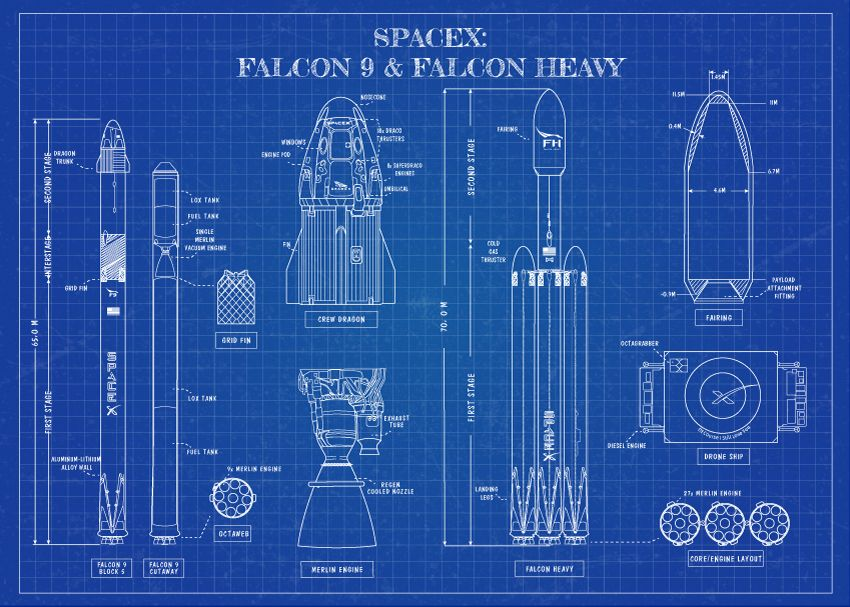
\includegraphics[width=0.4\textwidth]{gambar/cetakbiru.jpg}

  % Ubah sesuai dengan keterangan gambar yang diinginkan.
  \caption{Cetak biru roket yang akan diuji coba. \cite{cetakbiruspacex}}
  \label{fig:cetakbiru}
\end{figure}

\lipsum[9-10]

\subsection{Lorem Ipsum}
\label{subsec:loremipsum}

\lipsum[11]

% Contoh pembuatan tabel.
\begin{table}
  \caption{Contoh tabel sederhana}
  \label{tab:tabelsederhana}
  \centering
  \begin{tabular}{lll}
    \toprule
    Heading1 & Heading2 & Heading3 \\
    \midrule
    One      & Two      & Three    \\
    Four     & Five     & Six      \\
    \bottomrule
  \end{tabular}
\end{table}

% Contoh pembuatan potongan kode.
\begin{lstlisting}[
  language=C++,
  caption={Program halo dunia.},
  label={lst:halodunia}
]
#include <iostream>

int main() {
    std::cout << "Halo Dunia!";
    return 0;
}
\end{lstlisting}

\lipsum[12]

% Contoh pembuatan daftar.
\begin{enumerate}
  \item \lipsum[13][1-4]
  \item \lipsum[13][5-8]
  \item \lipsum[13][9-12]
\end{enumerate}

\lipsum[14-15]

% Ubah judul dan label berikut sesuai dengan yang diinginkan.
\section{Result and Discussion}
\label{sec:resultanddiscussion}

% Ubah paragraf-paragraf pada bagian ini sesuai dengan yang diinginkan.
\subsection{Model Performance Testing using Confusion Matrix}

In this research, the Convolutional Neural Network (CNN) method is used to create a model. During CNN model building, image data is collected and grouped which is then used as a dataset for CNN model training and validation. The data trained in the form of eye landmark images that have been grouped into five classes as described in the methodology. The five classes that classify the eye landmark image data are “Right” (\emph{"Kanan"}), “Left” (\emph{"Kiri"}), “Forward” (\emph{"Maju"}), “Backward” (\emph{"Mundur"}), and “Stop”. The dataset used in this research consists of 2000 image data. Furthermore, in each class folder, the 400 image data is divided (split) with a weight of 70\% for training data so that there are 280 image data entered in the training folder and 30\% weight for validation data so that there are 120 image data entered in the validation folder. The visualization of the dataset used can be seen in Figure \ref{fig:dataset}.

\begin{figure} [ht] \centering
  % Nama dari file gambar yang diinputkan
  \includegraphics[scale=0.38]{gambar/bab4/visual.png}
  % Keterangan gambar yang diinputkan
  \caption{Dataset Visual Diagram}
  % Label referensi dari gambar yang diinputkan
  \label{fig:dataset}
\end{figure}

In model building, the training process is carried out using a CNN model consisting of eleven layers with 32 filters in the first layer, 64 filters in the second layer, and 128 filters in the third layer as the structure described in the research methodology. Training on the CNN model is done with a configuration of 40 epoch stages with 10 training steps per epoch. The early stopping module is also added during model training in order to obtain the best model, which is at the 30th epoch. Based on the training results, an accuracy value of 100\% is generated with a validation accuracy of 99.83\%. In addition, the training results also show a loss value of 0.22\% with a validation loss of 1.14\%. These variables can be seen in Figure \ref{fig:acc_loss} which has visualized the results of accuracy and validation accuracy as well as the results of loss and loss validation in graphical form with the values of accuracy, validation accuracy, loss, and loss validation against each stage of epoch.

\begin{figure}[H]
  \centering
  \subfloat[Accuracy]{
    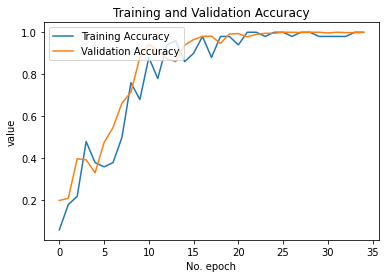
\includegraphics[width=0.23\textwidth]{gambar/bab4/model5 (30cm)/train.png}
    %\caption{30 sentimeter}
    \label{fig:imageaccu}}
    \hfil 
  \subfloat[Loss]{
    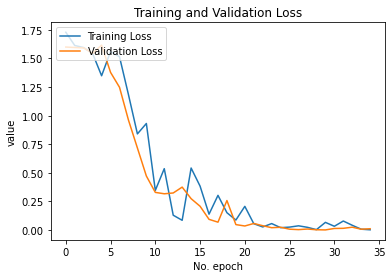
\includegraphics[width=0.23\textwidth]{gambar/bab4/model5 (30cm)/loss.png}
    %\caption{50 sentimeter}
    \label{fig:imageloss}}

  \caption{Graph of Accuracy and Loss on the Model Training Results}
  \label{fig:acc_loss}
\end{figure}

After obtaining the accuracy and loss for the model training results, the next calculation is done for confusion matrix. The confusion matrix is calculated by comparing the actual label (true label) with the predicted label and then the two labels will be visualized into a matrix divided into each control class, where predicted label becomes the X-axis and true label becomes the Y-axis. From the visualization of confusion matrix from Figure \ref{fig:confuse}, it can be observed that there is a prediction error in the “Forward"  (\emph{"Maju"}) class.

\begin{figure} [H] \centering
  % Nama dari file gambar yang diinputkan
  \includegraphics[scale=0.5]{gambar/bab4/modelkedua/modelkedua.png}
  % Keterangan gambar yang diinputkan
  \caption{Model Confusion Matrix}
  % Label referensi dari gambar yang diinputkan
  \label{fig:confuse}
\end{figure}

Then from confusion matrix, we get classification results that can be grouped into several parameters, namely true positive, true negative, false positive, and false negative. True positive is the result where the model correctly predicts the positive class. Similarly, true negative is the result where the model correctly predicts the negative class. The positive class is the class itself, while the negative class is any class other than itself. False positive is the result where the model incorrectly predicts the positive class. And false negative is the result where the model incorrectly predicts the negative class. The classification results can be seen in Table \ref{tb:cm_model}.

%Tabel 4.2
\begin{table}[H]
  \caption{Model Validation Results}
  \label{tb:cm_model} 
  \centering
  \begin{tabular}{|l|c|c|c|c|}
  \hline
  \rowcolor[HTML]{C0C0C0} 
  \textbf{Class} & \textbf{TP} & \textbf{TN} & \textbf{FP} & \textbf{FN} \\ \hline
  Right    & 120          & 479         & 1           & 0           \\ \hline
  Left      & 120          & 480         & 0           & 0           \\ \hline
  Forward      & 119          & 480         & 0           & 1           \\ \hline
  Backward     & 120          & 480         & 0           & 0           \\ \hline
  Stop  & 120          & 480         & 0           & 0           \\ \hline
  \end{tabular}
\end{table}

From the classification results, the model validation value can then be calculated. The validation values calculated are accuracy, precision, recall, and f-1 score. A more detailed description can be seen in Table \ref{tb:vs_model}. It can be seen that the model has a high average accuracy value of 99.93\% with an average precision value of 99.83\%, average recall of 99.83\%, and average f-1 score of 99.83\%. This indicates that the model has a high level of accuracy in predicting eye poses.

%Tabel 4.3
\begin{table}[H]
  \caption{Model Validation Results}
  \label{tb:vs_model} 
  \centering
  \begin{tabular}{|l|c|c|c|c|}
  \hline
  \rowcolor[HTML]{C0C0C0} 
  \textbf{Class} & \textbf{Accuracy} & \textbf{Precision} & \textbf{Recall} & \textbf{F1-Score} \\ \hline
  Right    & 99.83\%            & 99.17\%             & 100\%           & 99.59\%            \\ \hline
  Left     & 100\%          & 100\%           & 100\%           & 100\%           \\ \hline
  Forward      & 99.83\%          & 100\%           & 99.17\%          & 99.58\%          \\ \hline
  Backward     & 100\%            & 100\%             & 100\%           & 100\%            \\ \hline
  Stop  & 100\%            & 100\%             & 100\%           & 100\%            \\ \hline
  \end{tabular}
\end{table}

\subsection{Model Performance Testing using Distance Variations}

In this test scenario, the model is tested based on several distance variations. Distance testing is useful to determine the performance and accuracy of the model if the input image is taken from different distances. This needs to be tested because the further the distance of the image detector, the smaller the visual image data obtained. The distance validation results used are 30 centimeters which can be seen in Table \ref{tb:30cm}, 50 centimeters in Table \ref{tb:50cm}, 70 centimeters in Table \ref{tb:70cm}, and 90 centimeters in Table \ref{tb:90cm}. For an example of the distance test variation dataset can be seen in Figure \ref{fig:Variasi Jarak Kamera}.

\begin{figure}[H]
  \centering
  \subfloat[30 centimeters]{
    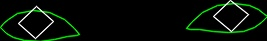
\includegraphics[width=0.2\textwidth]{gambar/bab4/30.jpg}
    %\caption{30 sentimeter}
    \label{fig:imagea}}
    \hfil 
  \subfloat[50 centimeters]{
    
\includegraphics[width=0.2\textwidth]{gambar/bab4/50.jpg}
    %\caption{50 sentimeter}
    \label{fig:imageb}}

  \subfloat[70 centimeters]{
    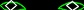
\includegraphics[width=0.2\textwidth]{gambar/bab4/70.jpg}
    %\caption{70 sentimeter}
    \label{fig:imagec}}
    \hfil
  \subfloat[90 centimeters]{
    
\includegraphics[width=0.2\textwidth]{gambar/bab4/90.jpg}
    %\caption{90 sentimeter}
    \label{fig:imaged}}

  \caption{Camera Distance Variations}
  \label{fig:Variasi Jarak Kamera}
\end{figure}

\begin{table}[ht]
  \caption{Model Validation Results with a Distance of 30 cm}
  \label{tb:30cm}
  \centering
  \begin{tabular}{|l|c|c|c|c|}
  \hline
  \rowcolor[HTML]{C0C0C0} 
  \textbf{Class} & \textbf{Accuracy} & \textbf{Precision} & \textbf{Recall} & \textbf{F1-Score} \\ \hline
  Right    & 100\%            & 100\%             & 100\%           & 100\%            \\ \hline
  Left     & 100\%          & 100\%           & 100\%           & 100\%           \\ \hline
  Forward      & 100\%          & 100\%           & 100\%          & 100\%          \\ \hline
  Backward     & 100\%            & 100\%             & 100\%           & 100\%            \\ \hline
  Stop  & 100\%            & 100\%             & 100\%           & 100\%            \\ \hline
  \end{tabular}
\end{table}

\begin{table}[ht]
  \caption{Model Validation Results with a Distance of 50 cm}
  \label{tb:50cm}
  \centering
  \begin{tabular}{|l|c|c|c|c|}
  \hline
  \rowcolor[HTML]{C0C0C0} 
  \textbf{Class} & \textbf{Accuracy} & \textbf{Precision} & \textbf{Recall} & \textbf{F1-Score} \\ \hline
  Right    & 100\%            & 100\%             & 100\%           & 100\%            \\ \hline
  Left     & 100\%          & 100\%           & 100\%           & 100\%           \\ \hline
  Forward      & 100\%          & 100\%           & 100\%          & 100\%          \\ \hline
  Backward     & 100\%            & 100\%             & 100\%           & 100\%            \\ \hline
  Stop  & 100\%            & 100\%             & 100\%           & 100\%            \\ \hline
  \end{tabular}
\end{table}

\begin{table}[H]
  \caption{Model Validation Results with a Distance of 70 cm}
  \label{tb:70cm}
  \centering
  \begin{tabular}{|l|c|c|c|c|}
  \hline
  \rowcolor[HTML]{C0C0C0} 
  \textbf{Class} & \textbf{Accuracy} & \textbf{Precision} & \textbf{Recall} & \textbf{F1-Score} \\ \hline
  Right    & 100\%            & 100\%             & 100\%           & 100\%            \\ \hline
  Left     & 100\%          & 100\%           & 100\%           & 100\%           \\ \hline
  Forward      & 99.50\%          & 100\%           & 97.50\%          & 98.73\%          \\ \hline
  Backward     & 99.50\%            & 97.56\%             & 100\%           & 98.77\%            \\ \hline
  Stop  & 100\%            & 100\%             & 100\%           & 100\%            \\ \hline
  \end{tabular}
\end{table}

\begin{table}[H]
  \caption{Model Validation Results with a Distance of 90 cm}
  \label{tb:90cm}
  \centering
  \begin{tabular}{|l|c|c|c|c|}
  \hline
  \rowcolor[HTML]{C0C0C0} 
  \textbf{Class} & \textbf{Accuracy} & \textbf{Precision} & \textbf{Recall} & \textbf{F1-Score} \\ \hline
  Right    & 100\%            & 100\%             & 100\%           & 100\%            \\ \hline
  Left     & 100\%          & 100\%           & 100\%           & 100\%           \\ \hline
  Forward      & 96.67\%          & 94.64\%           & 88.33\%          & 91.38\%          \\ \hline
  Backward     & 96.67\%            & 89.06\%             & 95\%           & 91.94\%            \\ \hline
  Stop  & 100\%            & 100\%             & 100\%           & 100\%            \\ \hline
  \end{tabular}
\end{table}
    
\subsection{Model Performance Testing using Lighting Variations}

In eye pose-based wheelchair control systems, lighting variations have a significant influence on the performance of the detection model. The purpose of this test is to evaluate the success and failure rate of the model in detecting eye poses in three lighting conditions, such as dark lighting (35 Lux) which can be seen in Table \ref{tb:lux35}, dim (55 Lux) in Table \ref{tb:lux55}, and bright (131 Lux) in Table \ref{tb:lux131}. The type of lighting tested was ambient light, which simulates ambient lighting with different intensity variations. For lighting test variations can be seen in Figure \ref{fig:Variasi Pencahayaan}.

\begin{figure}[H]
  \centering
  \subfloat[35 Lux]{
    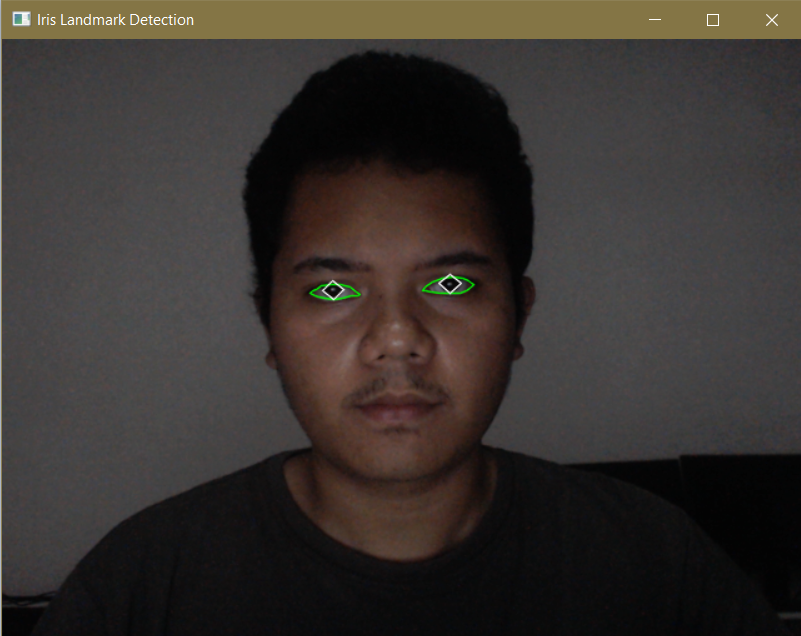
\includegraphics[width=0.15\textwidth]{gambar/bab4/33.png}
    %\caption{30 sentimeter}
    \label{fig:imageaa}}
  \hfil
  \subfloat[55 Lux]{
    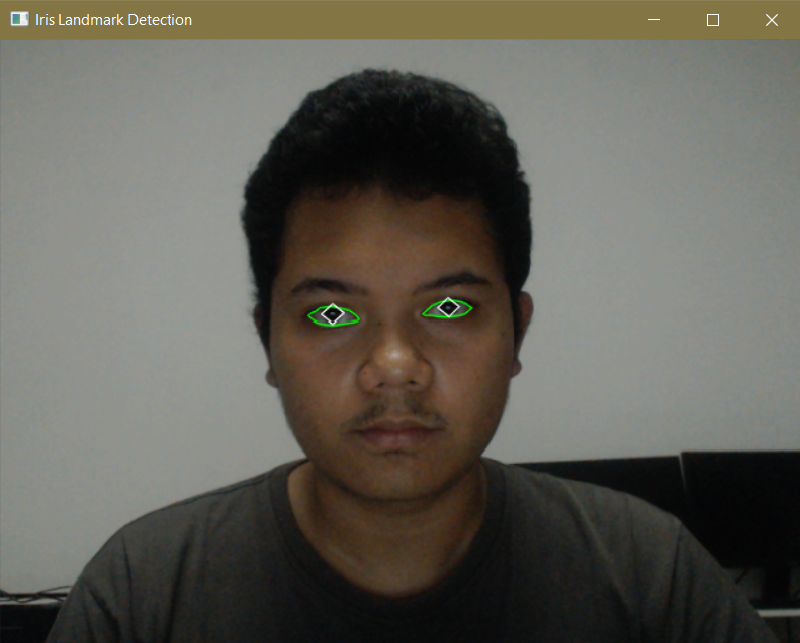
\includegraphics[width=0.15\textwidth]{gambar/bab4/55.png}
    %\caption{50 sentimeter}
    \label{fig:imagebb}}

  \subfloat[131 Lux]{
    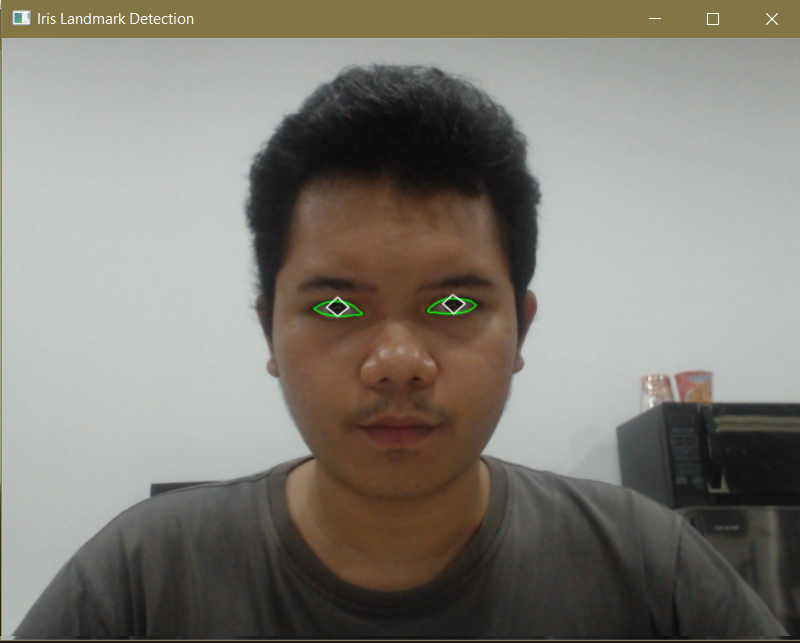
\includegraphics[width=0.15\textwidth]{gambar/bab4/131.png}
    %\caption{70 sentimeter}
    \label{fig:imagecc}}

  \caption{Lighting Variations}
  \label{fig:Variasi Pencahayaan}
\end{figure}

\begin{table}[ht]
  \caption{Model Testing with 35 Lux Lighting}
  \label{tb:lux35} 
  \centering
  \begin{tabular}{|l|c|c|}
  \hline
  \rowcolor[HTML]{C0C0C0} 
  \textbf{Class} &  \multicolumn{1}{c|}{\textbf{\begin{tabular}[c]{@{}c@{}}Percentage of  \\ Success\end{tabular}}} & \multicolumn{1}{c|}{\textbf{\begin{tabular}[c]{@{}c@{}}Percentage of\\ Unsuccess\end{tabular}}} \\ \hline
  Right                                                                                                                                                                             & 100\%                                                                                   & 0\%                                                                                         \\ \hline
  Left                                                                                                                                                                               & 100\%                                                                                   & 0\%                                                                                         \\ \hline
  Forward                                                                                                                                                                              & 90\%                                                                                    & 10\%                                                                                        \\ \hline
  Backward                                                                         & 93.33\%                                                                                 & 6.67\%                                                                                      \\ \hline
  Stop                                                                                          & 100\%                                                                                   & 0\%                                                                                         \\ \hline
\end{tabular}
\end{table}

\begin{table}[ht]
  \caption{Model Testing with 55 Lux Lighting}
  \label{tb:lux55} 
  \centering
  \begin{tabular}{|l|c|c|}
  \hline
  \rowcolor[HTML]{C0C0C0} 
  \textbf{Class} &  \multicolumn{1}{c|}{\textbf{\begin{tabular}[c]{@{}c@{}}Percentage of  \\ Success\end{tabular}}} & \multicolumn{1}{c|}{\textbf{\begin{tabular}[c]{@{}c@{}}Percentage of\\ Unsuccess\end{tabular}}} \\ \hline
  Right                                                                                                                                                                             & 100\%                                                                                   & 0\%                                                                                         \\ \hline
  Left                                                                                                                                                                               & 100\%                                                                                   & 0\%                                                                                         \\ \hline
  Forward                                                                                                                                                                              & 96.67\%                                                                                    & 3.33\%                                                                                        \\ \hline
  Backward                                                                         & 93.33\%                                                                                 & 6.67\%                                                                                      \\ \hline
  Stop                                                                                          & 100\%                                                                                   & 0\%                                                                                         \\ \hline
\end{tabular}
\end{table}

\begin{table}[H]
  \caption{Model Testing with 131 Lux Lighting}
  \label{tb:lux131} 
  \centering
  \begin{tabular}{|l|c|c|}
  \hline
  \rowcolor[HTML]{C0C0C0} 
  \textbf{Class} &  \multicolumn{1}{c|}{\textbf{\begin{tabular}[c]{@{}c@{}}Percentage of  \\ Success\end{tabular}}} & \multicolumn{1}{c|}{\textbf{\begin{tabular}[c]{@{}c@{}}Percentage of\\ Unsuccess\end{tabular}}} \\ \hline
  Right                                                                                                                                                                             & 100\%                                                                                   & 0\%                                                                                         \\ \hline
  Left                                                                                                                                                                               & 100\%                                                                                   & 0\%                                                                                         \\ \hline
  Forward                                                                                                                                                                              & 100\%                                                                                    & 0\%                                                                                        \\ \hline
  Backward                                                                         & 100\%                                                                                 & 0\%                                                                                      \\ \hline
  Stop                                                                                          & 100\%                                                                                   & 0\%                                                                                         \\ \hline
\end{tabular}
\end{table}

\subsection{Frame Per Second (FPS) Performance Testing on Wheelchair Control System}

The Frame Per Second (FPS) performance test aims to evaluate the speed of the system in processing eye poses in real-time to control the wheelchair. FPS is an important indicator in assessing the smoothness and responsiveness of the system, especially in applications that require pose detection and fast decision making. The FPS test results on the laptop and NUC can be seen in Table \ref{tb:fps}.

\begin{table}[H]
  \caption{FPS Performance Results on Laptop and NUC}
  \label{tb:fps}
  \centering
  \begin{tabular}{|l|c|c|}
  \hline
  \rowcolor[HTML]{C0C0C0} 
  \textbf{Class} &  \multicolumn{1}{c|}{\textbf{\begin{tabular}[c]{@{}c@{}}Average \\ FPS on Laptop\end{tabular}}} & \multicolumn{1}{c|}{\textbf{\begin{tabular}[c]{@{}c@{}}Average\\ FPS on NUC\end{tabular}}} \\ \hline
  Right           & 12.745              & 10.567           \\ \hline
  Left           & 12.635              & 10.617            \\ \hline
  Forward           & 13.078              & 10.068           \\ \hline
  Backward           & 13.507              & 9.734           \\ \hline
  Stop           & 12.580              & 10.127            \\ \hline
  \end{tabular}
\end{table}

\subsection{Inference Time on Model and Response Time on Wheelchair Motor Testing}

The Inference Time test on the model and Response Time test on the wheelchair motor aim to evaluate how fast the eye pose-based wheelchair control system can respond to commands from the user. Inference Time measures the time taken by the model to detect and classify eye poses, while Response Time measures the time taken for the wheelchair motor to start moving after receiving a signal from the model. The time test results of Inference Time and Response Time can be seen in Table \ref{tb:response}.

\begin{table}[H]
  \caption{Inference Time and Response Time Testing Results}
  \label{tb:response}
  \centering
  \begin{tabular}{|l|c|c|}
  \hline
  \rowcolor[HTML]{C0C0C0} 
  \textbf{Class} &  \multicolumn{1}{c|}{\textbf{\begin{tabular}[c]{@{}c@{}}Average \\ Inference Time (s)\end{tabular}}} & \multicolumn{1}{c|}{\textbf{\begin{tabular}[c]{@{}c@{}}Average\\ Response Time (s)\end{tabular}}} \\ \hline
  Right           & 0.0626             & 0.2328           \\ \hline
  Left           & 0.0640              & 0.0933            \\ \hline
  Forward           & 0.0656               & 0.4337           \\ \hline
  Backward           & 0.0637              & 0.1409           \\ \hline
  Stop           & 0.0666              & 0.4318            \\ \hline
  \end{tabular}
\end{table}

\subsection{Stability of Wheelchair Motor Testing}

The stability test on the wheelchair motor aims to ensure that the output time executed by the motor remains stable for each input given by the user through the eye pose control system. This involves measuring the time taken by the motor to respond to each eye pose command and ensuring that the response time remains consistent across different input conditions. The results of the motor stability test can be seen in Table \ref{tb:stabil}.

\begin{table}[H]
  \caption{Motor Stability Testing Results}
  \label{tb:stabil}
  \centering
  \begin{tabular}{|l|c|c|}
  \hline
  \rowcolor[HTML]{C0C0C0} 
  \textbf{Class} &  \multicolumn{1}{c|}{\textbf{\begin{tabular}[c]{@{}c@{}}Average \\ Motor Running Time (s)\end{tabular}}} \\ \hline
  Right          & 6.013                        \\ \hline
  Left           & 6.469                          \\ \hline
  Forward           & 6.532                         \\ \hline
  Backward         & 6.863                         \\ \hline
  Stop           & 4.933                          \\ \hline
  \end{tabular}
\end{table}
% Ubah judul dan label berikut sesuai dengan yang diinginkan.
\section{Conclusion}
\label{sec:conclusion}

% Ubah paragraf-paragraf pada bagian ini sesuai dengan yang diinginkan.

\lipsum[21-23]

% Acknowledgment jika ada
%\section{Acknowledgement}
\label{sec:acknowledgement}

The authors would like to thank the Ministry of Research, Technology, and Higher Education of the Republic of Indonesia for \lipsum[1]

% Menampilkan daftar pustaka dengan format IEEE
\bibliographystyle{IEEEtranN}
\bibliography{pustaka/pustaka.bib}

% Menyeimbangkan bagian akhir di kedua kolom
\balance

\end{document}
